\documentclass{article}
\usepackage{bm}
\usepackage{amsmath}
\usepackage{graphicx}
\usepackage{mdwlist}
\usepackage[colorlinks=true]{hyperref}
\usepackage{geometry}
\usepackage{kotex}
\geometry{margin=1in}
\geometry{headheight=2in}
\geometry{top=2in}
\usepackage{palatino}
%\renewcommand{\rmdefault}{palatino}
\usepackage{fancyhdr}
%\pagestyle{fancy}
\rhead{}
\lhead{}
\chead{%
  {\vbox{%
      \vspace{2mm}
      \large
      Hardware System Design 4190.309A\hfill
\\
      Seoul National University
      \\[4mm]
      \textbf{Practice \#2. SW app on MNIST}\\
      \textbf{Sangjun Son, Jiwon Lee}
    }
  }
}


\usepackage{paralist}

\usepackage{todonotes}
\setlength{\marginparwidth}{2.15cm}

\usepackage{tikz}
\usetikzlibrary{positioning,shapes,backgrounds}

\begin{document}
\pagestyle{fancy}

\section*{Goal}

\begin{itemize*}
\item Implement matrix vector(MV) multiplication in C++.
\item Integrate MV multiplication into the pretrained model (MLP).
\begin{itemize*}
\item On MNIST
\end{itemize*}
\end{itemize*}

\section{MV Multiplication}

\begin{figure}[ht]
	\centering
	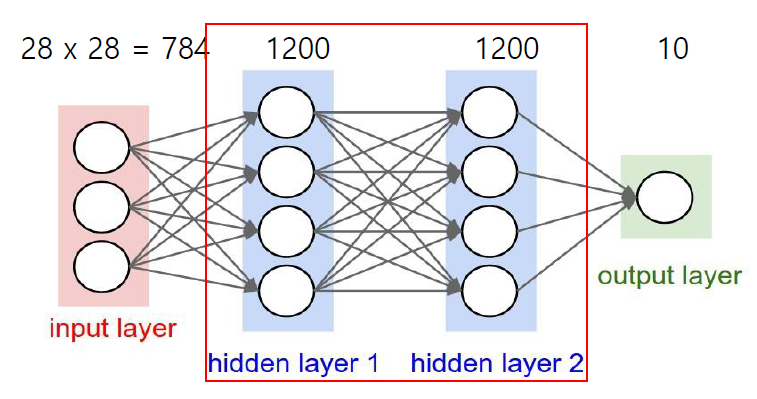
\includegraphics[width=0.7\textwidth]{fig1.png}
	\caption{MNIST MLP에 각각의 layer 사이의 perceptron 간 모든 연결에 대한 weight matrix와 이전 layer까지 연산된 벡터와의 곱셈이 이뤄진다. 빨간색으로 표시된 부분에서 1200 x 1200 크기의 행렬과 1200 크기의 벡터와의 가장 큰 연산이 이뤄진다. }
\label{fig1}
\end{figure}

\subsection*{Tiling Method}

MNIST 문제에서 주어지는 숫자 이미지 크기는 28 x 28 크기의 이미지이며 이를 벡터화 하여 여러 MLP를 거쳐 마지막에 output layer에 10개의 숫자 중 나타날 확률을 학습하게 된다. Figure~\ref{fig1}에서 표현하듯이 행렬과 벡터 곱셈이 매우 크므로 공간이나 시간적 복잡도를 최적화하기 위해서는 Tiling method를 사용하게 된다. 행렬과 벡터를 일정한 크기로 나누어 가속기를 통해 쓰레드를 나누어 빠른 연산 속도를 가능하게 한다.\\
\\
행렬의 각각의 조각과 대응되는 input 벡터도 쪼개고 block operation (단순 행렬 곱셈을 수행)을 수행하게 된다. Figure~\ref{fig2}에서처럼 $M_{SIZE}$ x $V_{SIZE}$ 크기의 행렬과 $V_{SIZE}$의 input vector를 행렬 연산한 후 $M_{SIZE}$ 크기의 output 벡터에 연산된 결과값을 누적한다. 이 과정을 모든 타일에 대해서 수행하게 되면 최종적으로 큰 행렬 벡터 곱셈을 수행하는 것과 같은 결과가 나오게 된다.

\begin{figure}[ht]
	\centering
	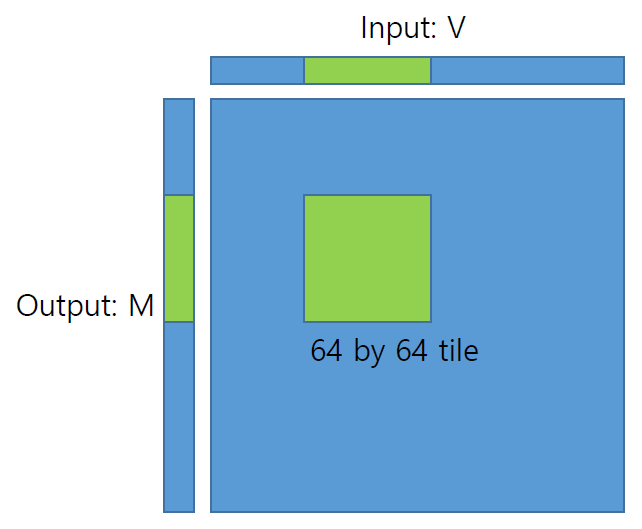
\includegraphics[width=0.45\textwidth]{fig2.png}
	\caption{Tiling method: 큰 행렬과 벡터 연산에 있어서 작은 영역으로 나누어 이에 대한 행렬 벡터 곱셈을 진행한 후 차곡차곡 더하는 과정을 진행하게 된다. 이 때 행렬에서 일정한 부분으로 자른 조각의 크기는 $M_{SIZE}$ x $V_{SIZE}$ 이다. 위의 경우 $M_{SIZE} = V_{SIZE} = 64$ 이다.}
\label{fig2}
\end{figure}

\newpage
\section{Implementation}

행렬 벡터 연산을 수행할 때는 작은 크기의 행렬 벡터 연산 (Tiling)으로 축소 대응시켜 계산을 하게 되는데 이 때 자주 사용되는 함수가 block operation이다. 함수를 사용하기 위해서 중간 중간에 data\_라는 데이터 중간 저장소를 통해 곱셈에 사용될 행렬과 벡터를 fetching 하고 연산된 output vector를 덮어쓰는 과정을 반복하게 된다. \\
\\
아래와 같이 (1) Tile의 크기를 지정하는 초기화, (2) 데이터 중간 저장소에 작은 input 벡터와 (3) 행렬을 기존의 데이터 위에 덮어쓰고, (4) block op를 수행한 뒤에 (5) 마지막으로, data\_에서 작은 output 벡터를 fetch 한 후에 최종 결과에 누적하는 과정을 거치게 된다.
		
\subsection{Initialize input vector}
\label{sec:initialize}
%int block_row = min(m_size_, num_output-i);
%int block_col = min(v_size_, num_input-j);          
$M_{SIZE}$와 $V_{SIZE}$에 해당하는 만큼의 행렬과 벡터를 가리키는 block\_row 와 block\_col이라는 변수를 통해 block 단위의 MV 연산을 진행 부분을 지칭한다. 이 때 주목해야 하는 점은 타일이 모두 행렬과 벡터를 꽉 채워 연산을 진행할 수 있지만 그렇지 않은 경우가 존재한다는 것이다. 즉, 초기에 곱셈을 해야 하는 행렬의 세로 크기가 $M_{SIZE}$의 배수가 아니거나 가로 크기가 $V_{SIZE}$의 배수가 아닐 수 있기 때문에 margin 연산을 해야하는 것이다.

\subsection{Assign a vector}
\label{sec:vector}
%            for (int col = 0; col < block_col; col++)
%                data_[col] = input[j + col];
%           for (int col = block_col; col < v_size_; col++)
%                data_[col] = 0;
앞서 이야기 했듯이 block operation을 수행하는 부분에서 곱셈을 하는 부분을 data\_라는 중간 저장소를 통해 벡터와 행렬을 가져온다. 그렇기 때문에 block operation을 호출하기 전 곱셈을 수행할 행렬과 벡터를 data\_ 위에 올려놓는 작업을 진행한다. 현 section에서는 block\_col 크기의 벡터를 입력시키는 과정을 소개한다.\\
\\
이 때 block operation에서는 입력되는 벡터의 크기가 어떻든 $M_{SIZE}$와 $V_{SIZE}$에 해당하는 만큼의 행렬과 벡터 연산을 진행하기 때문에 block\_col이 $V_{SIZE}$ 보다 작은 상황을 고려해주어야 한다. 그렇지 않다면 전 step에서 사용되었던 벡터 값이 잘못된 연산 결과를 초래할 수 있기 때문이다. 해법으로는 $M_{SIZE} -$(block\_col) 만큼의 부분을 0으로 덮어쓰는 방법이 있을 것이다.

\subsection{Assign a matrix}
%            for (int row = 0; row < block_row; row++)
%                for (int col = 0; col < block_col; col++)
%                    data_[(row+1)*v_size_ + col] = large_mat[(i+row)*num_input + (j+col)];
Section~\ref{sec:vector}에서 소개되었던 것처럼 data\_에 벡터를 추가한 뒤에는 행렬을 추가하게 된다. 원본 행렬에 있는 값들을 참조시켜 1차원 배열로 flatten하여 덮어쓰기를 진행한다.

\subsection{Execute block MV multiplication \& Accumulate intermediate results}
\label{sec:accumulate}
%			const float* ret = this->blockMV();
%			for(int row = 0; row < block_row; ++row)
%			{
%				output[i + row] += ret[row];
%			}
중간 저장소에 있는 작은 벡터와 행렬을 fetch하여 block operation을 수행하고 연산결과를 data\_의 앞 부분에 올려놓는다.
연산 결과 block\_row 크기의 ret 벡터를 최종 결과 벡터에 누적을 한다.  이 모든 과정 Section~\ref{sec:initialize} \~{} \ref{sec:accumulate}을 모든 타일에 대해 cover 될 때까지 진행한다.


\section{Experiment}
주어진 large\_mat 과 input 에서 가장 기본적인 행렬과 벡터의 곱셈은 Equation~\ref{eqn1}과 같이 나타난다.
위의 방법으로 Tiling 없이 실행시켰을 때 결과는 Figure~\ref{fig3}과 같다.
\begin{equation}
\label{eqn1}
	output_{ij} = \sum^n_{k=1} large\_mat_{ik} \cdot input_{kj}
\end{equation}

\begin{figure}[ht]
	\centering
	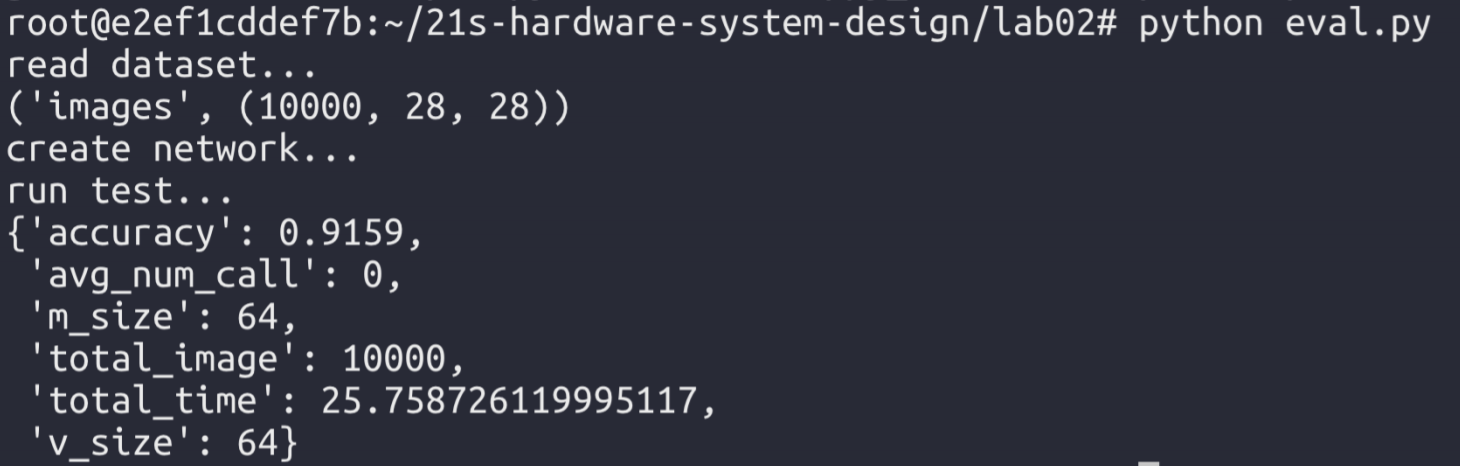
\includegraphics[width=0.9\textwidth]{fig3.png}
	\caption{Result without Tiling}
\label{fig3}
\end{figure}

\newpage
행렬과 벡터의 곱셈에서, 행렬과 벡터를 작은 크기로 나누어 곱 연산을 수행하고 결과값을 누적하여 최종 값을 구한다. 
Figure~\ref{fig4}은 블록 크기 ($M_{SIZE}$, $V_{SIZE}$) : (64, 64), (16, 16), (8, 16), (16, 8) 에 대하여 수행한 결과이다.

\begin{figure}[ht]
	\centering
	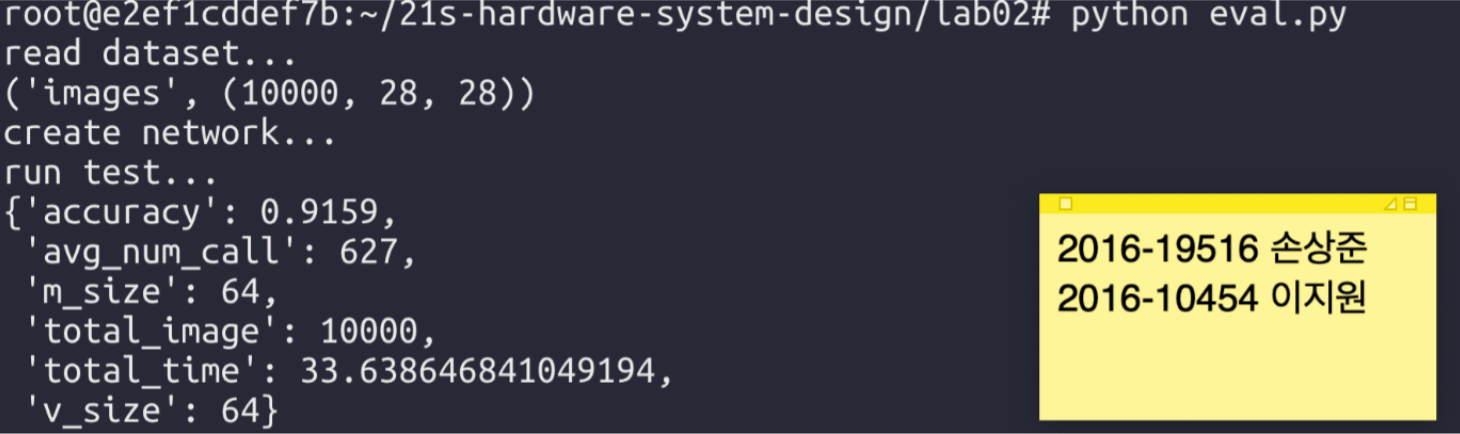
\includegraphics[width=0.75\textwidth]{fig4.png}
	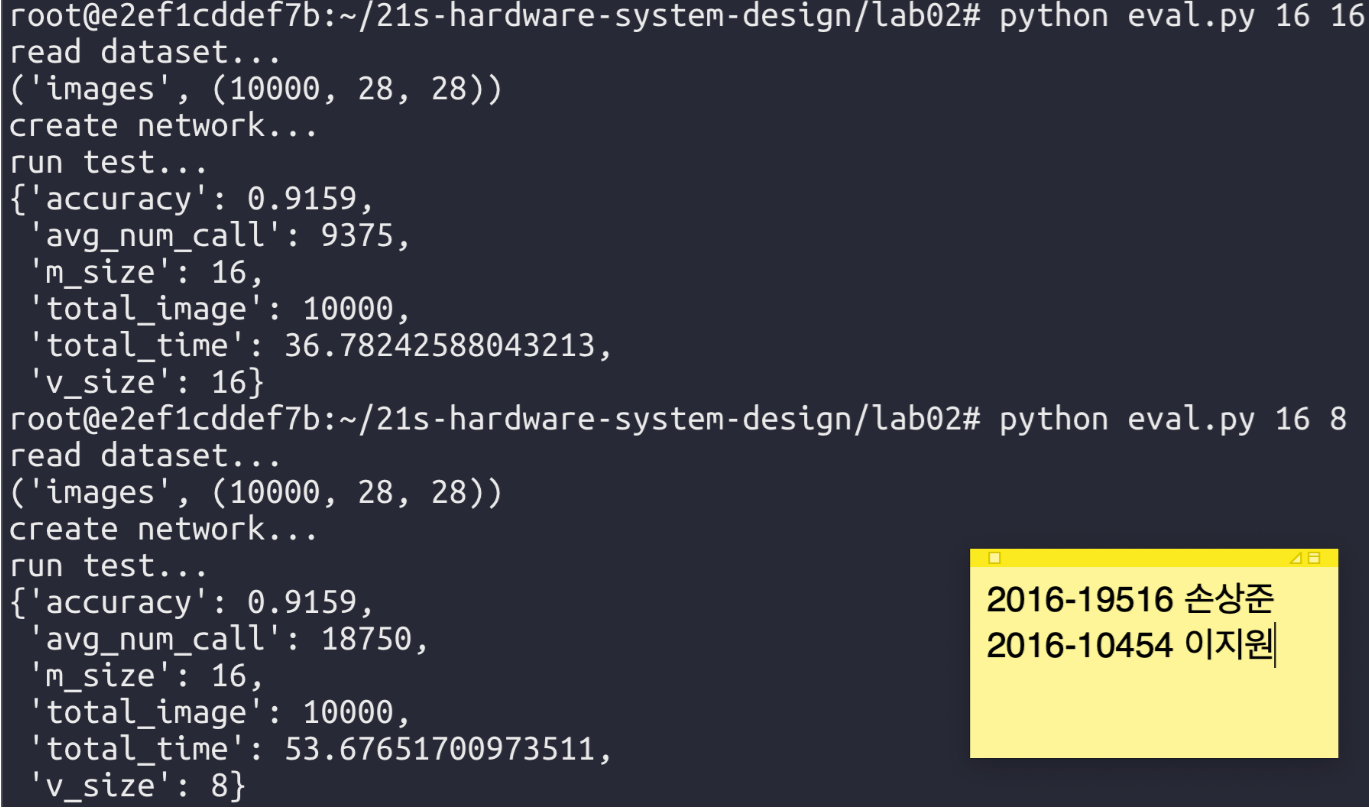
\includegraphics[width=0.75\textwidth]{fig5.png}
	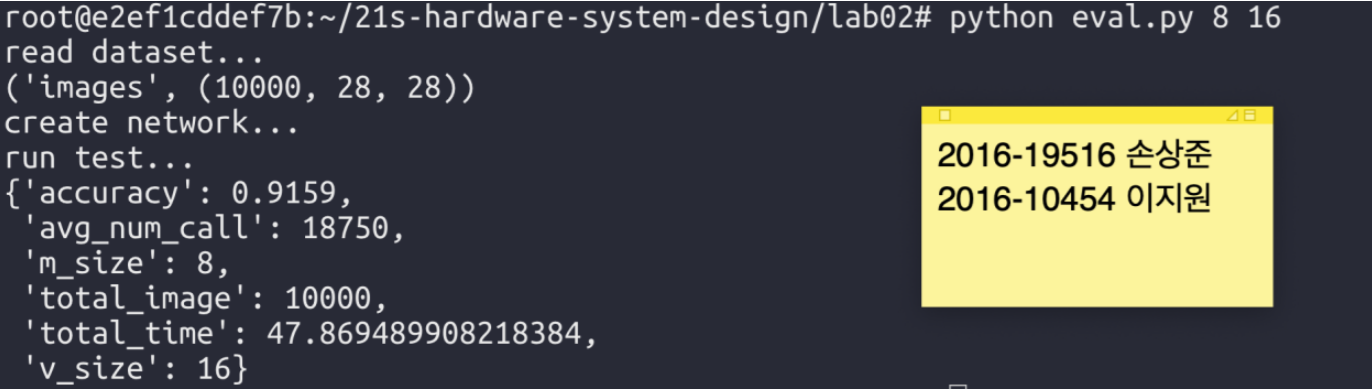
\includegraphics[width=0.75\textwidth]{fig6.png}
	\caption{Result with (64, 64), (16, 16), (8, 16), (16, 8) Tiling}
\label{fig4}
\end{figure}

연산 쓰레드를 증가하거나 다른 accelerator 없이 한 개의 머신에서 $M_{SIZE}$와 $V_{SIZE}$를 변화하였을 때 걸리는 시간을 비교하였다. 어떤 방식으로 나누더라도 모든 행렬 연산 결과는 동일하게 도출되었으며 MNIST 데이터 셋에 대하여 약 91.59\%의 정확도를 보였다. Figure~\ref{fig7}에서 볼 수 있듯이, $M_{SIZE}$와 $V_{SIZE}$를 각각 $2^1$ 부터  $2^{10}$ 까지 달리하여 측정하였다. 가장 적은 시간을 보였던 결과는 $M_{SIZE}=16$, $V_{SIZE}=32$ 일 때, 약 23.02 초가 소요되었다.

\begin{figure}[ht]
	\centering
	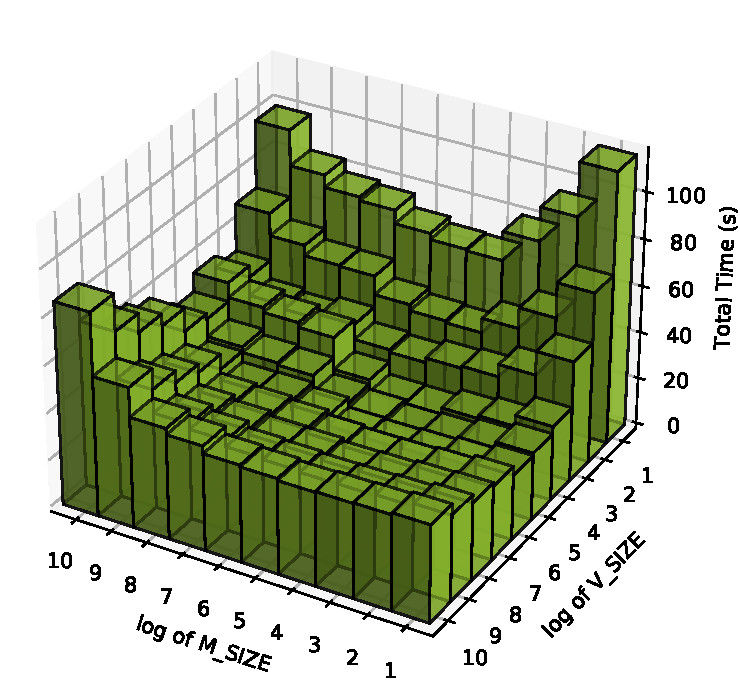
\includegraphics[width=0.7\textwidth]{fig7.pdf}
	\caption{한 대의 머신에서 $M_{SIZE}$와 $V_{SIZE}$를 변화하였을 때 걸리는 시간을 비교한 결과이며 단순히 block 크기를 키우거나 줄인다고 연산 속도가 개선되거나 오래 걸리지 않음을 확인할 수 있다.}
\label{fig7}
\end{figure}

\newpage
\section{Conclusion}
결과를 관찰하였을 때, 동일한 training set이 사용되어 정확도는 모두 같고, $M_{SIZE}$과 $V_{SIZE}$의 크기가 클수록 전체 시간이 줄어드는 것을 확인할 수 있었다.
비록 이번 랩에서는 28 x 28의 비교적 크기가 작은 행렬을 이용하였지만, FPGA 보드가 64 x 64 크기의 행렬과 벡터의 곱셈을 지원하기 때문에, 크기가 큰 행렬, 벡터의 곱셈을 계산해야 하는 경우 위의 방법이 필수적일 것이라는 생각이 들었다.
또한, 이러한 방법이 더 빠르게 행렬과 벡터의 곱셈 결과를 얻는 데도 사용될 수 있다고 생각하였다.
Tiling 방법에서 각 tile들의 곱셈은 서로 독립적이기 때문에, multi-thread를 이용하여 계산하게 되면 더 빠르게 결과값을 도출할 수 있다고 생각한다.

\end{document}
